\begin{mynotitleposter}

    \headerbox
    {Глава 3. Движение 1}
    {name=first,column=0,row=0,span=3}
    {
        {\huge\bf
            \vspace{-15pt}
            \begin{figure}[H]
                \begin{equation*}\begin{array}{ccc}
                    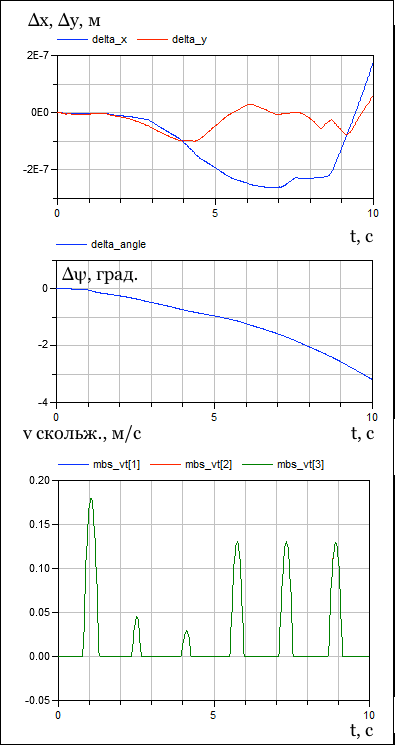
\includegraphics[width=0.3\textwidth, 
                    trim=10 20 10 450,
                    clip]{content/parts/3_friction/diploma/img/res/comparison_v_0_0_omega_1_frac_1e-1_n_4_time_10s.png} 
                    &
                    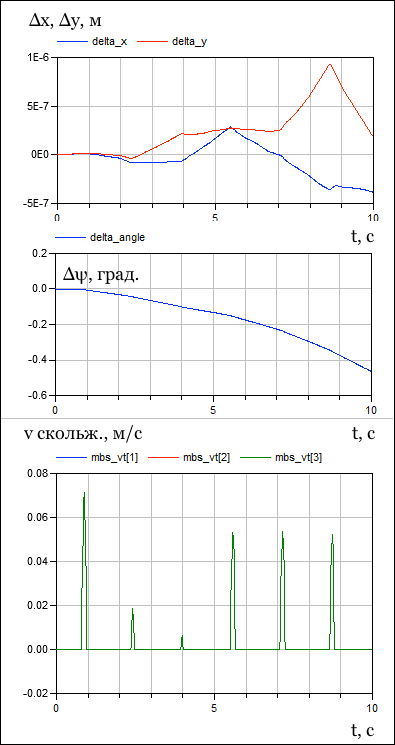
\includegraphics[width=0.3\textwidth, 
                    trim=10 20 10 450,
                    clip]{content/parts/3_friction/diploma/img/res/comparison_v_0_0_omega_1_frac_1e-2_n_4_time_10s.png}
                    &
                    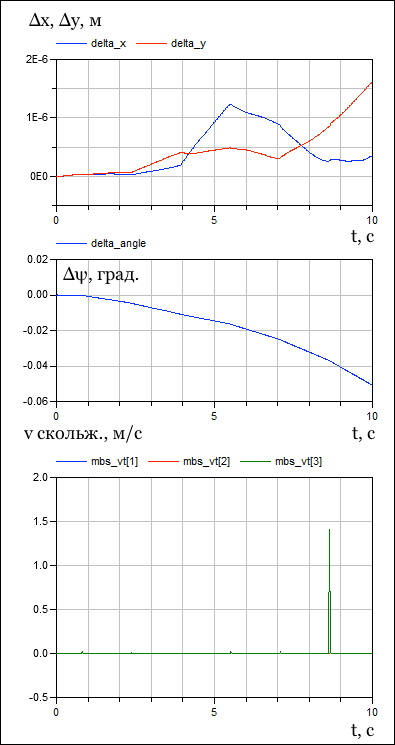
\includegraphics[width=0.3\textwidth,
                    trim=10 20 10 450,
                    clip]{content/parts/3_friction/diploma/img/res/comparison_v_0_0_omega_1_frac_1e-3_n_4_time_10s.png} 
                    \\
                    \ddfrac{m_{\text{рол}}}{m_{\text{к}}} = 10^{-1}, v_0 = 0, \omega_0 = 1 &
                    \ddfrac{m_{\text{рол}}}{m_{\text{к}}} = 10^{-2}, v_0 = 0, \omega_0 = 1 &
                    \ddfrac{m_{\text{рол}}}{m_{\text{к}}} = 10^{-3}, v_0 = 0, \omega_0 = 1
                    \\
                \end{array}\end{equation*}
            \end{figure}
            \vspace{-45pt}
            \begin{figure}[H]
                \begin{equation*}\begin{array}{ccc}
                    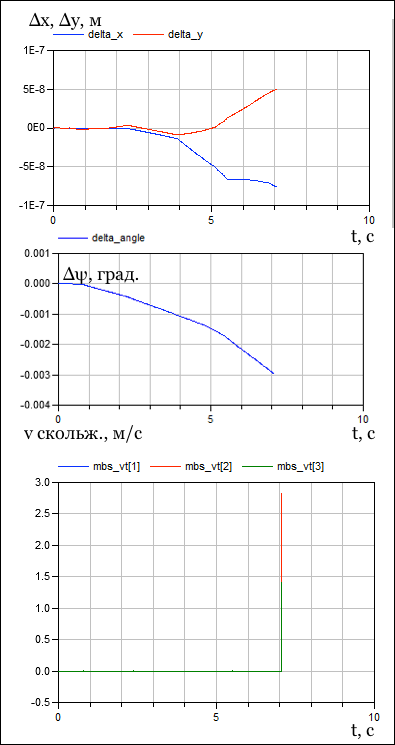
\includegraphics[width=0.3\textwidth, 
                    trim=10 20 10 450,
                    clip]{content/parts/3_friction/diploma/img/res/comparison_v_0_0_omega_1_frac_1e-4_n_4_time_10s.png}
                    &
                    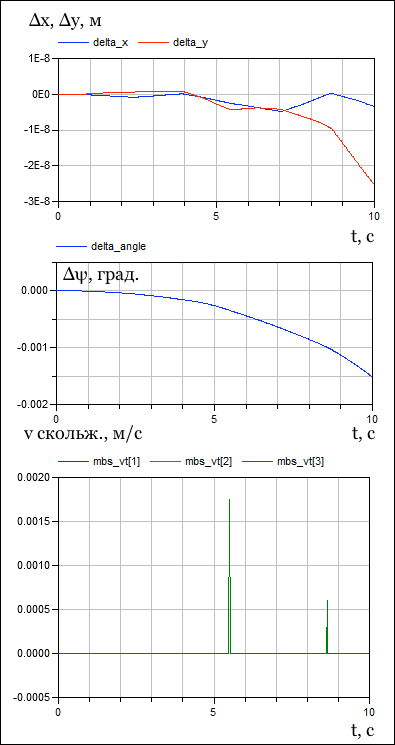
\includegraphics[width=0.3\textwidth, 
                    trim=10 20 10 450,
                    clip]{content/parts/3_friction/diploma/img/res/comparison_v_0_0_omega_1_frac_1e-5_n_4_time_10s.png}
                    &
                    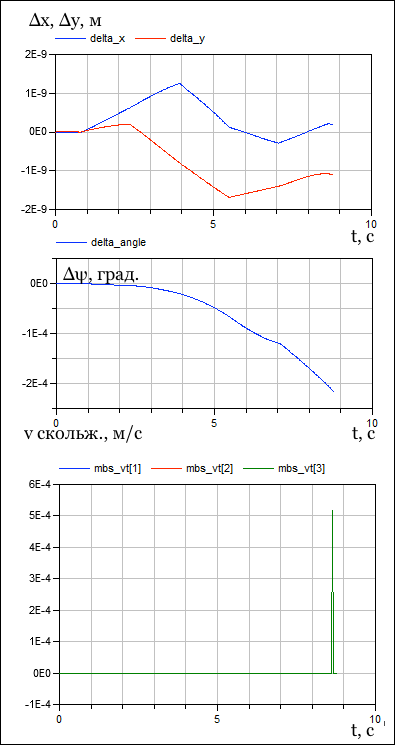
\includegraphics[width=0.3\textwidth, 
                    trim=10 20 10 450,
                    clip]{content/parts/3_friction/diploma/img/res/comparison_v_0_0_omega_1_frac_1e-6_n_4_time_10s.png}
                    \\
                    \ddfrac{m_{\text{рол}}}{m_{\text{к}}} = 10^{-4}, v_0 = 0, \omega_0 = 1 &
                    \ddfrac{m_{\text{рол}}}{m_{\text{к}}} = 10^{-5}, v_0 = 0, \omega_0 = 1 &
                    \ddfrac{m_{\text{рол}}}{m_{\text{к}}} = 10^{-6}, v_0 = 0, \omega_0 = 1
                    \\
                \end{array}\end{equation*}
            \end{figure}
        }
    }
    
    \headerbox
    {Глава 3. Движение 2}
    {name=second,column=0,row=1,below=first,span=3}
    {
        {\huge\bf
            \begin{figure}[H]
                \begin{center}\begin{equation*}\begin{array}{ccc}
                    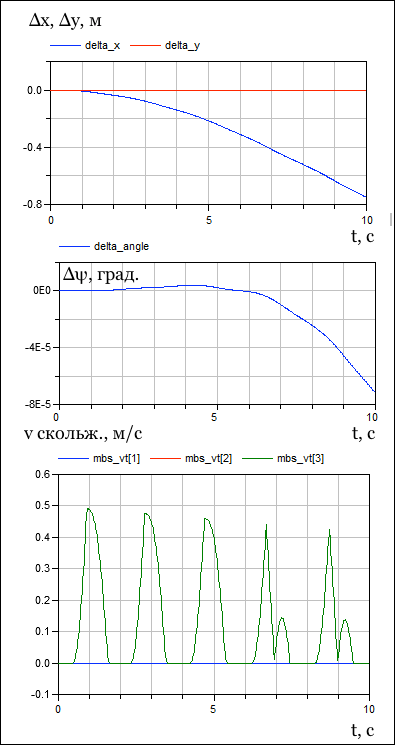
\includegraphics[width=0.3\textwidth, 
                    trim=10 20 10 450,
                    clip]{content/parts/3_friction/diploma/img/res/comparison_v_1_0_omega_0_frac_1e-1_n_4_time_10s.png}
                    &
                    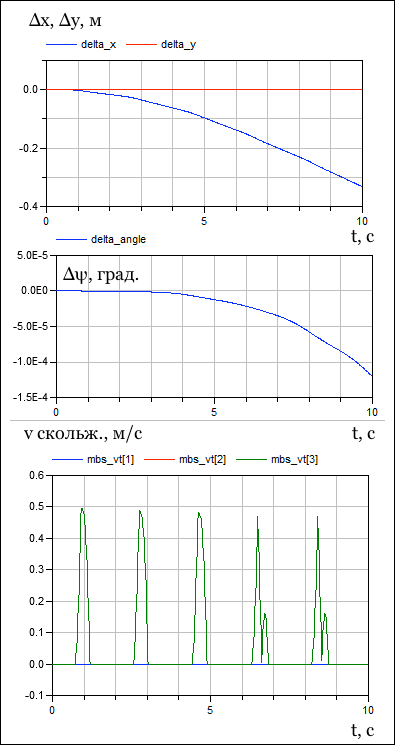
\includegraphics[width=0.3\textwidth, 
                    trim=10 20 10 450,
                    clip]{content/parts/3_friction/diploma/img/res/comparison_v_1_0_omega_0_frac_1e-2_n_4_time_10s.png}
                    &
                    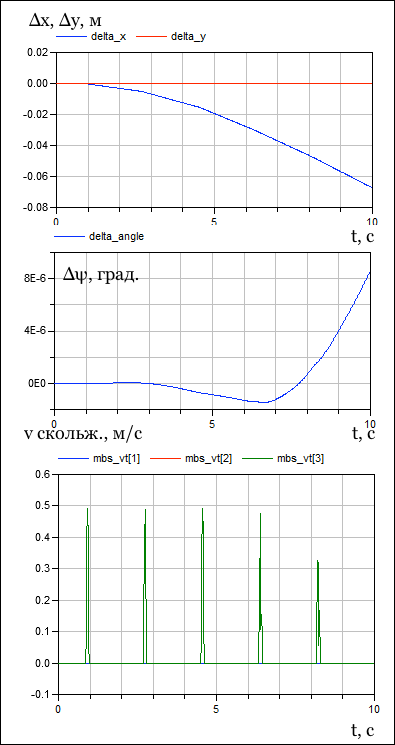
\includegraphics[width=0.3\textwidth, 
                    trim=10 20 10 450,
                    clip]{content/parts/3_friction/diploma/img/res/comparison_v_1_0_omega_0_frac_1e-4_n_4_time_10s.png}
                    \\
                    \ddfrac{m_{\text{рол}}}{m_{\text{к}}} = 10^{-1}, v_0 = 1, \omega_0 = 0 &
                    \ddfrac{m_{\text{рол}}}{m_{\text{к}}} = 10^{-2}, v_0 = 1, \omega_0 = 0 &
                    \ddfrac{m_{\text{рол}}}{m_{\text{к}}} = 10^{-4}, v_0 = 1, \omega_0 = 0
                    \\
                \end{array}\end{equation*}\end{center}
            \end{figure}
        }
    }
    
    \headerbox
    {Глава 3. Сравнение с безынерционной моделью}
    {name=third,column=0,row=2,below=second,span=3}
    {
        \qquad
        \minipage{0.5\textwidth}
            {\huge\bf
                \begin{tabular}{l|l|l}
                     & Движение $1$ & Движение $2$ \\ \hline
                    $\frac{m_{\text{рол}}}{m_{\text{к}}}$ &
                    $\Delta \theta$ &
                    $\max(|\Delta x|, |\Delta y|)$ \\ \hline
                    $10^{-1}$ & $\approx 1$       & $\approx 1$       \\
                    $10^{-2}$ & $\approx 10^{-1}$ & $\approx 0.5$     \\
                    $10^{-3}$ & $\approx 10^{-2}$ & $\approx 10^{-1}$ \\
                    $10^{-4}$ & $\approx 10^{-3}$ & $\approx 10^{-2}$ \\
                    $10^{-5}$ & $\approx 10^{-3}$ &                   \\
                    $10^{-6}$ & $\approx 10^{-4}$ & 
                \end{tabular}
            }
        \endminipage
        \qquad
        \minipage{0.4\textwidth}
            {\huge
                Проведено сравнение движений безынерционной модели экипажа и модели экипажа на плоскости с сухим трением.
                В таблице приведены величины отличий угла курса $\theta$ экипажа и координат центра масс $x, y$ к моменту безразмерного времени $t = 10$.
                Отличия уменьшаются с уменьшением порядка величины отношения массы одного ролика $m_{\text{рол}}$ к суммарной массе колеса $m_{\text{к}}$.
            }
        \endminipage
    }
    
\end{mynotitleposter}


